% Based on Diagram of Android activity life cycle
\documentclass[border=10pt]{standalone}
\usepackage{tikz}
\usetikzlibrary{arrows.meta,shapes, calc}
\tikzset{%
  >={Latex[width=2mm,length=2mm]},
  % Specifications for style of nodes:
            base/.style = {rectangle, rounded corners, draw=black,
                           minimum width=4cm, minimum height=1.5cm,
                           text centered, font=\sffamily},
  separateModel/.style = {base, fill=blue!20},
         process/.style = {base, minimum width=2.5cm, fill=orange!15},
}
\begin{document}    
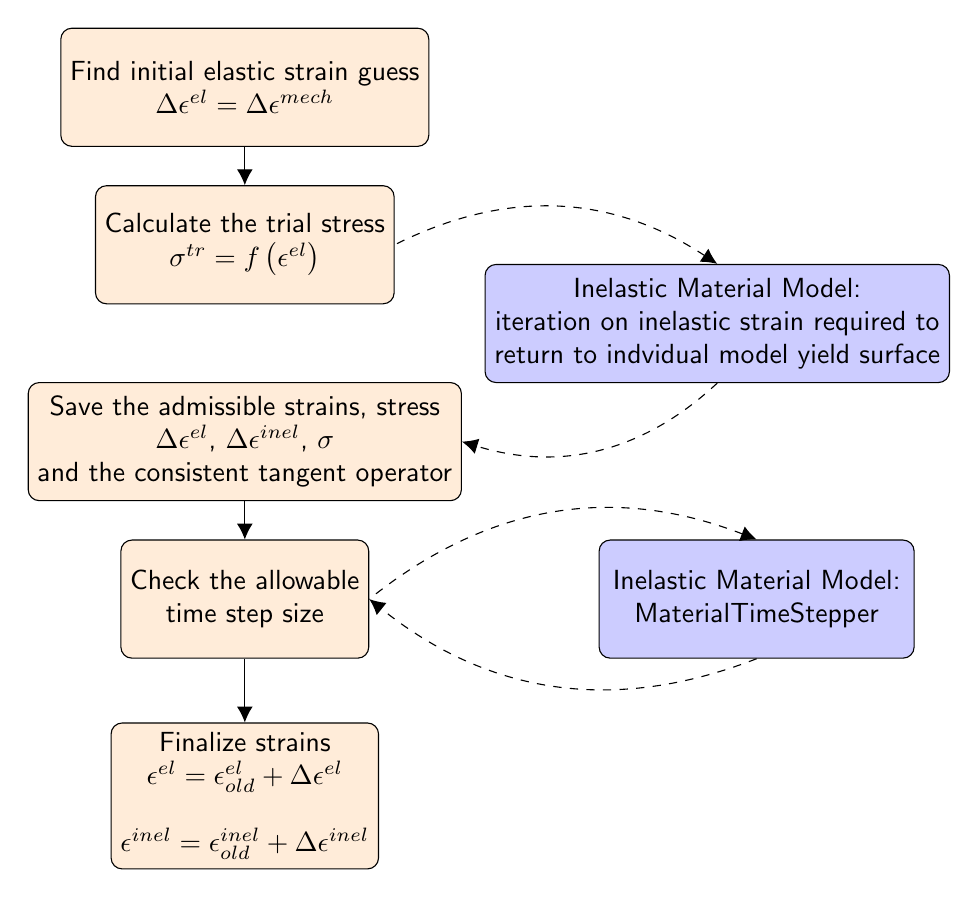
\begin{tikzpicture}[node distance=1.5cm,
    every node/.style={fill=white, font=\sffamily}, align=center]
  % Specification of nodes (position, etc.)
  \node (start)               [process]
                              {Find initial elastic strain guess \\ $\Delta \epsilon^{el} = \Delta \epsilon^{mech}$};
  \node (trialStressBlock)    [process, below of=start, yshift=-0.5cm]
                              {Calculate the trial stress \\
                              $\sigma^{tr} = f \left( \epsilon^{el} \right)$};
  \node (matAdmissibleBlock)  [separateModel, right of=trialStressBlock, xshift=4.5cm, yshift=-1cm]
                              {Inelastic Material Model: \\ iteration on inelastic strain required to \\ 
                              return to indvidual model yield surface};  
  \node (admissiblesBlock)    [process, below of=trialStressBlock, yshift=-1cm]
                              {Save the admissible strains, stress \\
                              $\Delta \epsilon^{el}$, $\Delta \epsilon^{inel}$, $\sigma$\\
                              and the consistent tangent operator};                            

  \node (matTimeStepBlock)    [process, below of=admissiblesBlock, yshift=-0.5cm] 
                              {Check the allowable \\ time step size};
                              
  \node (materialTimeStepper) [separateModel, right of=matTimeStepBlock, xshift=5cm]
                              {Inelastic Material Model: \\ MaterialTimeStepper};
  \node (finalizeStrainBlock) [process, below of=matTimeStepBlock, yshift=-1cm] 
                              {Finalize strains \\
                              $\epsilon^{el} = \epsilon^{el}_{old} + \Delta \epsilon^{el}$ \\ 
                              \vspace{0.01cm} \\
                              $\epsilon^{inel} = \epsilon^{inel}_{old} + \Delta \epsilon^{inel}$};


 
  % Specification of lines between nodes specified above
  % with aditional nodes for description 
  \draw[->]                   (start) to (trialStressBlock);

  \draw[<-, bend right=30, dashed] (matAdmissibleBlock.north) to (trialStressBlock.east);
  \draw[->, bend left=30, dashed]  (matAdmissibleBlock.south) to (admissiblesBlock.east);
  
  \draw[->]        (admissiblesBlock) to (matTimeStepBlock);
  \draw[->]        (matTimeStepBlock) to (finalizeStrainBlock);
  
  \draw[<-, bend right=30, dashed] (materialTimeStepper.north) to (matTimeStepBlock.east);
  \draw[->, bend left=30, dashed]  (materialTimeStepper.south) to (matTimeStepBlock.east);

  \end{tikzpicture}
\end{document}